\section{SYNTHETIC RECOVERY}
\label{app:synthetic}
\readorder{16}

\paragraph{Goal.} Check, on data simulated from the model's own generative story, that the final configuration recovers the planted intrinsic states, responses and gene programmes, that the adversary keeps the planted niche out of $\vz$, and how much a wrong leak fraction costs. A second simulation (\cref{app:planted-percell}) asks whether the response channel detects a per-cell response that the niche does not predict.

\paragraph{Generative process.} $N = 6{,}000$ cells uniformly in a $1{,}000\um$ box; $K = 8$ types assigned by a soft Voronoi partition around random anchors with Gumbel noise so that types cluster in space; the graph, kernel, composition and rings built by the same procedure as for real data from a Delaunay triangulation, with unit face lengths so that $\beta \propto \exp(-d/\tau)$ only; $\vz_i \sim \N(\mathbf{m}_{t_i}, 0.5^2\vI)$ with type means $\mathbf{m}_t \sim \N(\mathbf{0}, 1.5^2\vI)$; a planted response $\vw_i = \mathbf{M}^\top\vy_i + 0.3\,\boldsymbol\varepsilon_i$ linear in the true neighbour composition; $\log\vrho_i = \mathbf{A}\vz_i + \vB\vw_i$ (up to normalisation) with standard-normal loadings; $\rhobar_i$ the kernel-weighted neighbour average; $\vp_i$ the renormalised mixture at the planted $\kappa$; totals $\ell_i \sim \max(\Pois(150), 20)$; $\vx_i \sim \Mult(\ell_i, \vp_i)$; and a planted image descriptor $\vPhi_i = \mathbf{P}^\top\vy_i + 0.4\,\boldsymbol\varepsilon'_i$ in eight dimensions. $G = 60$ genes, planted $\dz = 4$, $\dw = 2$. Three worlds, drawn from three simulator seeds, at each planted $\kappa \in \{0, 0.2\}$.

\paragraph{Fit.} The final configuration (\cref{tab:architecture}), with the widths reduced to the small world ($\dz = 8$, $\dw = 2$, hidden width $128$, attention width $16$) and tiles of $512$ cells: the adversary at $\alphaa = 0.3$ with its composition term weighted three times, $\alphaw = 0.1$ with its warm-up over thirty epochs, $\alphaz = \tfrac12/\lbar$ with $\lbar$ the simulated section's median count ($150$, so $\alphaz \approx 0.0033$), $\omega = 1$, and the budget of $500$ epochs with patience $40$, with $15\%$ of the tiles held out for the stopping rule of \cref{sec:selection}. Every readout is taken on all cells at the accepted checkpoint. The uncontrolled arm is the same fit at $\alphaa = 0$. Each world is fitted with three model seeds, so every arm has nine fits. In the misspecified arms, the worlds planted at $\kappa = 0.2$ are fitted at each assumed $\kappa \in \{0, 0.1, 0.2, 0.3, 0.4\}$.

\paragraph{Readouts.} The agreement with the planted type, as the normalised mutual information between the planted types and a $k$-means clustering of $\vmu_z$ with $k = K$, against two references: the same clustering of the leading principal components of the log-normalised counts, which is what the counts alone support, and of the planted $\vz$ itself; the first canonical correlation between $\vmu_w$ and the planted response; the largest principal-angle cosine between the column spaces of the fitted and the planted loadings, against random two-dimensional subspaces of $\R^{60}$, whose cosine has a mean of $0.23$ and a $95$th percentile of $0.37$ to $0.38$ over $2{,}000$ draws; and the within-type coefficient of determination of the centred neighbour composition on $\vmu_z$, which is zero for the planted $\vz$.

\paragraph{Result.} \flag{TRIM}{long; the development-run bistability sentence is history, one clause suffices} At the matched leak fraction the final configuration recovers each planted quantity on every world (\cref{tab:synthetic}). The agreement of $\vmu_z$ with the planted type is $0.80$ to $0.96$, about what the counts support or more ($0.69$ to $0.93$; above the world's count clusters in seventeen fits of eighteen, and below them in one, $0.80$ against $0.83$) and short of the planted $\vz$ ($0.91$ to $0.98$), which is not reachable at $150$ counts per cell. The response correlates with the planted one at $0.83$ to $0.95$. The loadings are recovered above the random reference in every fit, at a cosine of $0.63$ to $0.99$; their recovery varies between seeds on some worlds, at both planted leak fractions (one fit of one world at $\kappa = 0$ reaches only $0.63$), which is why no gene-level statement on tissue is made from one fit (\cref{sec:sweep}). The intrinsic state carries almost none of the planted niche: the within-type $R^2$ of composition on $\vmu_z$ is at most $0.04$, against $0.11$ to $0.19$ without the adversary. Without the adversary the response and the loadings are also recovered worse and less reliably (canonical correlation $0.29$ to $0.91$, loadings $0.14$ to $0.85$). An earlier development run, at a configuration that is no longer used, had suggested that the loadings are bistable between seeds under a planted leak and stable without one; at the final configuration the spread between seeds is wider without a planted leak than under one: per world, the cosines span $0.63$ to $0.99$, $0.97$ to $0.99$ and $0.70$ to $0.98$ at $\kappa = 0$, against $0.98$ to $0.99$, $0.99$ and $0.77$ to $0.99$ at the matched $\kappa = 0.2$. Fitted at a wrong leak fraction, anywhere from $0$ to $0.4$ on worlds planted at $0.2$, the recovery moves little (\cref{fig:synthetic-misspec}): agreement $0.79$ to $0.97$, canonical correlation $0.78$ to $0.94$ (the lowest at an assumed $\kappa = 0$), loadings $0.71$ to $1.00$, composition $R^2$ at most $0.01$. On these worlds a leak fraction wrong by up to $0.2$ in either direction costs little of what is recovered. This also means that recovery does not point to the planted leak fraction, and it says nothing about leakage of a form the model cannot represent.

\paragraph{Simulator checks.} Leakage raises the kernel-weighted cosine between a cell's composition and its neighbours' by $0.22$ to $0.26$ at $\kappa = 0.4$ relative to $\kappa = 0$; the planted response is linearly predictable from composition ($R^2$ of $0.75$ to $0.87$); and the mixture is exactly the renormalised convex combination. These worlds have no isolated cells, so the reduction of the mixture to $\vrho$ for an isolated cell is not exercised here.

% Generated table: tab:synthetic. DO NOT EDIT BY HAND; regenerate instead.
% Command: python scripts/paper_tables.py
% Generated: 2026-10-01 17:35:54 (results frozen 2026-09-29 15:07:21, last line of scripts/logs/unassigned_2026-09-28/queue.log)
%
% Sources read (modification time):
%   data/datasets/synthetic_smoke/experiments/synthetic_recovery.json  (2026-09-29 16:58:56)  [after the freeze; see checks]
%
% Reading convention:
%   [min, max] over 3 world seeds x 3 model seeds per arm; best checkpoint; all 6,000 cells
%
% Provenance (row / column -> file : key):
%   every row: data/datasets/synthetic_smoke/experiments/synthetic_recovery.json : groups[arm, planted_kappa, assumed_kappa].fits[*] (min, max over world x model seeds; checked against the group's stored summary); references: world_references[planted kappa].<key> min, max over both planted kappa
%
% Checks and notes:
%   - Final arm configuration (config_final_arm): adv_comp_weight 3.0, alpha_w 0.1,
%     w_warmup_epochs 30, alpha_z 0.003333, epochs 500/patience 40, d_z 8, d_w 2, tile_cells
%     512, val_fraction 0.15. Simulator checks: all pass.
%   - Written 2026-09-29 16:58 (after the freeze; a new run,
%     scripts/logs/synthetic_2026-09-29/AGENT_REPORT.md).
%
% Pending cells:
%   none
%
\begin{table}[t]
\centering
\caption{Recovery on simulated sections, scaled to the simulated world: three worlds per planted \termSpillFrac{}, each fitted with three model seeds; the range over the 9 fits of each row. NMI of $\vmu_z$ with the planted type; \emph{CCA}: first canonical correlation of $\vmu_w$ with the planted response; \emph{Loadings}: principal-angle cosine of the fitted against the planted loadings; \emph{Comp.\ $R^2$}: within-type $R^2$ of neighbour composition from $\vmu_z$. Bold: the matched $\kappa$. \emph{References}: NMI of clusters of the counts and of the planted intrinsic state, composition $R^2$ of the planted state, and the loading cosine of a random subspace (mean and 95th percentile), each the range over the three worlds and both planted rates. A fit is stopped early on $15\%$ of held-out tiles; every read covers all cells. Arrows give the preferred direction.}
\label{tab:synthetic}
\small
\setlength{\tabcolsep}{3pt}
\begin{tabular}{@{}lcccc@{}}
\toprule
Arm & NMI, $\vmu_z$ $\uparrow$ & CCA, $\vw$ $\uparrow$ & Loadings $\uparrow$ & Comp.\ $R^2$ $\downarrow$ \\
\midrule
\multicolumn{5}{@{}l}{\emph{Assumed $\kappa$ = planted $\kappa$}} \\
\quad final configuration, $\kappa = 0$ & 0.80--0.96 & 0.85--0.95 & 0.63--0.99 & 0.00--0.04 \\
\quad without the adversary, $\kappa = 0$ & 0.71--0.94 & 0.29--0.91 & 0.14--0.78 & 0.11--0.19 \\
\quad final configuration, $\kappa = 0.2$ & 0.81--0.96 & 0.83--0.94 & 0.77--0.99 & 0.00--0.02 \\
\quad without the adversary, $\kappa = 0.2$ & 0.71--0.93 & 0.38--0.90 & 0.18--0.85 & 0.12--0.19 \\
\addlinespace
\multicolumn{5}{@{}l}{\emph{Planted $\kappa = 0.2$, final configuration, assumed $\kappa$:}} \\
\quad 0 & 0.86--0.96 & 0.78--0.94 & 0.75--0.96 & 0.00--0.01 \\
\quad 0.1 & 0.82--0.96 & 0.84--0.94 & 0.78--0.99 & 0.00--0.01 \\
\quad \textbf{0.2} & 0.81--0.96 & 0.83--0.94 & 0.77--0.99 & 0.00--0.02 \\
\quad 0.3 & 0.80--0.97 & 0.83--0.94 & 0.74--1.00 & 0.00--0.01 \\
\quad 0.4 & 0.79--0.97 & 0.83--0.94 & 0.71--1.00 & 0.00--0.01 \\
\addlinespace
\multicolumn{5}{@{}l}{\emph{References of the simulated worlds}} \\
\quad clusters of the counts & 0.69--0.93 & -- & -- & -- \\
\quad planted $\vz$ & 0.91--0.98 & -- & -- & 0.00 \\
\quad random subspace, mean & -- & -- & 0.23 & -- \\
\quad random subspace, 95th percentile & -- & -- & 0.37--0.38 & -- \\
\bottomrule
\end{tabular}
\end{table}


\begin{figure*}[t]
\centering
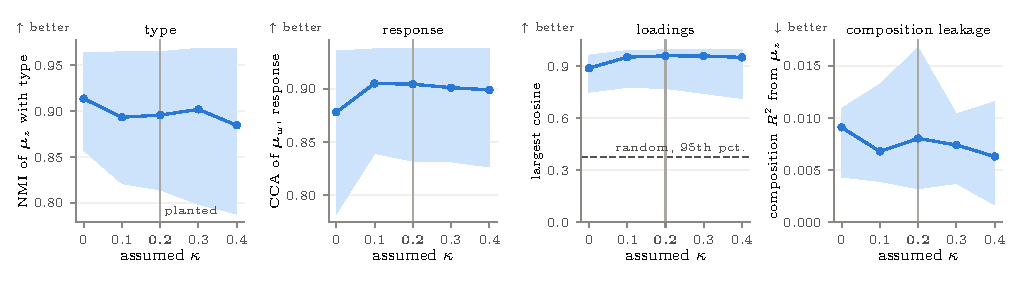
\includegraphics[width=\textwidth]{figures/fig_synthetic_misspec}
\caption{Recovery on the worlds simulated at $\kappa = 0.2$, fitted at each assumed $\kappa$: NMI of $\vmu_z$ with the planted type; the first canonical correlation of $\vmu_w$ with the planted response; the largest principal-angle cosine of the fitted against the planted loadings (dashed: the $95$th percentile of random subspaces); the within-type $R^2$ of neighbour composition on $\vmu_z$. Line: mean over nine fits, three worlds with three model seeds each; band: their range, which is mostly the spread between worlds. The vertical line marks the planted value. Arrows point toward the better direction. The values are in \cref{tab:synthetic}.}
\label{fig:synthetic-misspec}
\end{figure*}

\subsection{A Planted Per-Cell Response}
\label{app:planted-percell}

\flag{KEEP-CORE}{closes thread point 4: channel closed by design, not by the data} At the operating point the response posterior adds almost nothing on the four sections: about one part in a thousand of held-out reconstruction (\cref{tab:recon-modes}), and a per-cell divergence whose ranking of cells does not reproduce between seeds (\cref{app:kl-maps}). Either these tissues carry little per-cell response beyond what the niche predicts, or the weight $\alphaw = 0.1$ closes the channel whatever the data (\cref{sec:objective}). On tissue the two cannot be told apart, so we plant a per-cell response and ask whether the channel finds it.

\paragraph{The plant.} On the worlds planted at $\kappa = 0.2$ above, in $10\%$ of the cells of the most abundant type, drawn at random and therefore spread across niches, the log-rate is shifted along the first axis of the planted response programme, with norm $s$ times the size of the planted niche effect (the root mean square over cells of the planted niche shift of the log-rate), for $s \in \{0, 0.5, 1, 2\}$; $s = 0$ is the recovery world itself. The subset cannot be predicted from neighbour composition, nor from composition and the image descriptor: a five-fold cross-validated classifier within the planted type reaches an AUC of $0.44$ to $0.54$ on all three worlds. The shift lies inside the planted response programme deliberately. A per-cell shift unrelated to the niche is something the intrinsic state may legitimately carry, since the invariance only keeps the niche out of $\vz$; a shift along the response programme is a cell responding more or less strongly than its niche predicts, which is what the per-cell channel exists to carry. The fit is the final configuration unchanged, with three model seeds on world 0, and, as a replication outside the rule, on worlds 1 and 2.

\paragraph{The rule, fixed in advance.} The channel detects a response of strength $s$ if, on world 0, every seed separates the planted cells from the other cells of their type by their response divergence $\KL(q(\vw_i)\,\|\,p(\vw_i \mid \vc_i, t_i))$ with an AUC of at least $0.8$, and every pair of seeds ranks the cells' divergences with a Spearman correlation of at least $0.5$. The smallest $s$ detected was to be reported; if none were detected, that finding would be reported instead: at this weight the channel is closed by design, not by the data.

\paragraph{Result.} \flag{TRIM}{last four sentences repeat 3.5 and app:kl-maps} No strength is detected, on world 0 or on either replication (\cref{fig:planted-percell}, \cref{tab:planted-percell}). The divergence separates the planted cells only partly and not on every seed (AUC $0.66$ to $0.85$ at $s = 1$ and $0.56$ to $0.69$ at $s = 2$ on world 0), and a plant does not make the seeds agree more on the per-cell divergences: on world 0 they agree less at $s = 0.5$ and $s = 1$ than without a plant (Spearman $0.34$ to $0.36$ and $0.11$ to $0.18$, against $0.39$ to $0.41$ at $s = 0$) and about as much at $s = 2$ ($0.25$ to $0.42$); on world 1 they agree less at every strength, and on world 2 about as much as without a plant. The rule's agreement criterion is read over the whole map, and even the null does not reach it. The response's own deviation from its prior mean moves toward the plant, but weakly (correlation $0.11$ to $0.41$ for $s > 0$ over the three worlds), and the held-out gain from it on the planted cells stays below $0.02$ nats per count. As the plant grows, it is increasingly absorbed by the intrinsic state instead: read through the decoder along the planted direction, the correlation of $\vmu_z$ with the plant rises from at most $0.05$ at $s = 0$ to $0.36$ to $0.48$ on world 0, $0.86$ to $0.88$ on world 1 and $0.52$ to $0.70$ on world 2 at $s = 2$. At this weight the per-cell channel is therefore closed by design, not by the data: a per-cell response twice the size of the niche effect, planted where the model is meant to put it, is not found in the response's divergence, and much of it goes to $\vz$. On the four sections the response adds almost nothing to reconstruction beyond the context regression $\mpsi(\vc_i, t_i)$, and on three of them it also reads the merged sublabels as its prior mean does (on the lung section it separates some clusters better, \cref{app:subtype}); the absence of reproducible per-cell structure in its divergence there (\cref{app:kl-maps}) says nothing about whether the tissue has any. What opening the channel costs on tissue is in \cref{app:sensitivity}.

\begin{figure*}[t]
\centering
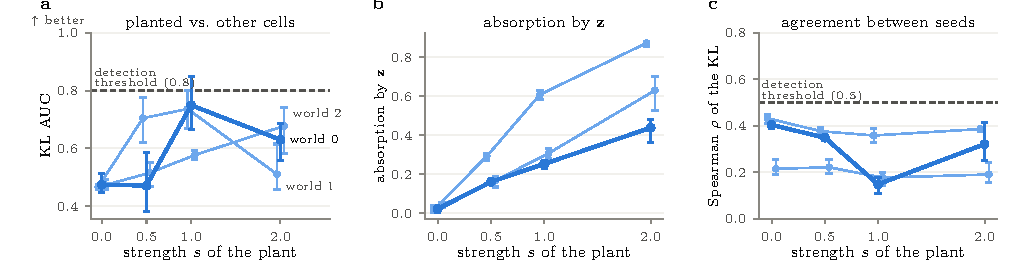
\includegraphics[width=\textwidth]{figures/fig_planted_percell}
\caption{The planted per-cell response against its strength $s$. \textbf{a},~KL AUC separating the planted cells from the other cells of their type by their response divergence; \textbf{b},~absorption of the plant by the intrinsic latent, read through the decoder along the planted direction; \textbf{c},~the Spearman correlation of the per-cell divergence between seeds. World 0, on which the rule fixed in advance decides, in bold; worlds 1 and 2, replications, lighter. Points: mean over three model seeds (seed pairs in c); bars: their range. Dashed: the rule's detection thresholds, a KL AUC of at least $0.8$ in every seed and a Spearman correlation of at least $0.5$ in every seed pair. Arrows point toward the better direction; absorption and the agreement between seeds have none. The values are in \cref{tab:planted-percell}.}
\label{fig:planted-percell}
\end{figure*}

% Generated table: tab:planted-percell. DO NOT EDIT BY HAND; regenerate instead.
% Command: python scripts/paper_tables.py
% Generated: 2026-09-30 11:59:21 (results frozen 2026-09-29 15:07:21, last line of scripts/logs/unassigned_2026-09-28/queue.log)
%
% Sources read (modification time):
%   data/datasets/synthetic_smoke/experiments/planted_percell.json  (2026-09-29 17:49:51)  [after the freeze; see checks]
%
% Reading convention:
%   [min, max] over model seeds 0-2 (seed pairs for Spearman and top-decile overlap) per world
%   and s
%
% Provenance (row / column -> file : key):
%   every row: data/datasets/synthetic_smoke/experiments/planted_percell.json : groups[world, s] per_seed[*] (KL AUC, w corr, z absorption, recon_gain_planted.gain_per_count) and cross_seed[*] (Spearman, top-decile overlap), min-max, checked against the group summary; detected from the group, checked against rule.by_s; predictability[world].*_auc
%
% Checks and notes:
%   - Written 2026-09-29 17:49 (after the freeze; a new run,
%     scripts/logs/planted_percell_2026-09-29/AGENT_REPORT.md). Smallest detected s on world 0:
%     None.
%
% Pending cells:
%   none
%
\begin{table}[t]
\centering
\caption{A planted per-cell response on simulated sections (planted $\kappa = 0.2$, final configuration unchanged). In $10\%$ of the cells of one type, spread across niches, the log-rate is shifted along the planted response programme by $s$ times the size of the planted niche effect (\emph{Shift}, its norm in log-rate units); $s = 0$ is the null. \emph{KL AUC}: the per-cell divergence of the response posterior from its prior separating the planted cells from the other cells of their type; \emph{$\vw$ corr.}: correlation of the response's deviation from its prior mean, along the planted direction, with the plant; \emph{$\vz$ absorption}: the same for the intrinsic latent, read through the decoder along the planted direction; \emph{Recon. gain}: held-out gain in nats per count of the full decode over the response at its prior mean, on planted cells; \emph{Spearman} and \emph{top-decile overlap}: agreement of the per-cell divergence between seeds. Ranges over three model seeds (seed pairs for the last two). The rule, fixed in advance and applied to world 0: the channel detects at $s$ if every seed has KL AUC $\geq 0.8$ and every seed pair a Spearman correlation $\geq 0.5$; worlds 1 and 2 replicate. No strength is detected. The planted subset cannot be predicted from neighbour composition or from composition and the image descriptor (five-fold cross-validated AUC 0.44--0.54 within the planted type, logistic and forest classifiers, all three worlds). The arrow gives the preferred direction.}
\label{tab:planted-percell}
\small
\setlength{\tabcolsep}{3pt}
\begin{tabular}{@{}lcccccccc@{}}
\toprule
$s$ & Shift & KL AUC $\uparrow$ & $\vw$ corr. & $\vz$ absorption & Recon. gain & Spearman & Top-decile overlap & Detected \\
\midrule
\multicolumn{9}{@{}l}{\emph{World 0 (decides)}} \\
\quad 0 & 0.0 & 0.45--0.51 & $-0.01$ to 0.01 & 0.00--0.03 & 0.002--0.006 & 0.39--0.41 & 0.42--0.46 & no \\
\quad 0.5 & 4.7 & 0.38--0.59 & 0.18--0.28 & 0.15--0.17 & 0.005--0.009 & 0.34--0.36 & 0.37--0.40 & no \\
\quad 1 & 9.3 & 0.66--0.85 & 0.34--0.37 & 0.23--0.27 & 0.008--0.017 & 0.11--0.18 & 0.21--0.31 & no \\
\quad 2 & 18.6 & 0.56--0.69 & 0.16--0.38 & 0.36--0.48 & 0.011--0.015 & 0.25--0.42 & 0.32--0.41 & no \\
\addlinespace
\multicolumn{9}{@{}l}{\emph{World 1 (replication)}} \\
\quad 0 & 0.0 & 0.46--0.48 & 0.02--0.04 & $-0.00$ to 0.04 & 0.003--0.006 & 0.41--0.45 & 0.34--0.38 & no \\
\quad 0.5 & 4.1 & 0.62--0.78 & 0.33--0.35 & 0.27--0.30 & 0.004--0.013 & 0.35--0.39 & 0.34--0.40 & no \\
\quad 1 & 8.1 & 0.67--0.80 & 0.32--0.41 & 0.58--0.63 & 0.004--0.013 & 0.33--0.39 & 0.39--0.42 & no \\
\quad 2 & 16.3 & 0.46--0.62 & 0.18--0.21 & 0.86--0.88 & 0.001--0.003 & 0.37--0.39 & 0.39--0.42 & no \\
\addlinespace
\multicolumn{9}{@{}l}{\emph{World 2 (replication)}} \\
\quad 0 & 0.0 & 0.46--0.49 & $-0.01$ to 0.05 & 0.03--0.05 & 0.000--0.001 & 0.19--0.25 & 0.23--0.28 & no \\
\quad 0.5 & 2.7 & 0.47--0.55 & 0.12--0.16 & 0.13--0.18 & 0.000--0.001 & 0.19--0.26 & 0.24--0.31 & no \\
\quad 1 & 5.5 & 0.56--0.59 & 0.11--0.29 & 0.28--0.33 & 0.002 & 0.14--0.20 & 0.23--0.25 & no \\
\quad 2 & 11.0 & 0.58--0.74 & 0.20--0.29 & 0.52--0.70 & 0.000--0.006 & 0.16--0.24 & 0.17--0.33 & no \\
\bottomrule
\end{tabular}
\end{table}

